\chapter{Formula Reference Card}
\label{ch:formula-reference-card}

\begin{nontechnical}
\textbf{This chapter is your quick-reference guide}---all the essential formulas for wireless communication system design in one place.

\textbf{What you'll find here:}
\begin{itemize}
\item Link budget calculations (path loss, power, antennas)
\item Signal quality metrics (SNR, $E_b/N_0$, BER)
\item Modulation formulas (symbol rates, spectral efficiency)
\item Error correction parameters
\item System design constants and conversions
\end{itemize}

\textbf{How to use it:} Each section groups related formulas with variable definitions and cross-references to detailed chapters. Worked examples demonstrate practical applications.
\end{nontechnical}

\section{Overview}

This reference card consolidates the most frequently used formulas in wireless communications system design. Each formula includes:
\begin{itemize}
\item Numbered equations for easy reference
\item Complete variable definitions
\item Units and typical value ranges
\item Cross-references to detailed derivations
\end{itemize}

\begin{keyconcept}
Use this reference card for \textbf{quick calculations} during system design. For theoretical background and detailed derivations, consult the cross-referenced chapters.
\end{keyconcept}

\section{Link Budget \& Propagation}\label{sec:link-budget-propagation}

\subsection{Friis Transmission Equation}
\label{sec:friis-equation}

The fundamental equation for received power in free space. See Chapter~\ref{ch:fspl} for derivation.

\textbf{Linear form:}
\begin{equation}
P_r = \frac{P_t G_t G_r \lambda^2}{(4\pi R)^2}
\label{eq:friis-linear}
\end{equation}
where:
\begin{itemize}
\item $P_r$ = Received power (W)
\item $P_t$ = Transmitted power (W)
\item $G_t$ = Transmit antenna gain (linear ratio)
\item $G_r$ = Receive antenna gain (linear ratio)
\item $\lambda$ = Wavelength (m)
\item $R$ = Distance (m)
\end{itemize}

\textbf{Logarithmic form (more practical):}
\begin{equation}
P_r\ (\text{dBm}) = P_t\ (\text{dBm}) + G_t\ (\text{dBi}) + G_r\ (\text{dBi}) - \text{FSPL}\ (\text{dB})
\label{eq:friis-db}
\end{equation}

\begin{calloutbox}{Why Use dB?}
The logarithmic form is preferred in practice because:
\begin{itemize}
\item Multiplications become additions
\item Large dynamic ranges (120+ dB) become manageable
\item Industry standard for link budgets
\item Calculator-friendly for field engineers
\end{itemize}
\end{calloutbox}

\subsection{Free-Space Path Loss (FSPL)}
\label{sec:fspl}

Path loss represents signal attenuation over distance in free space (no obstacles).

\textbf{Practical form (km and MHz):}
\begin{equation}
\text{FSPL}\ (\text{dB}) = 20\log_{10}(R) + 20\log_{10}(f) + 32.45
\label{eq:fspl-km-mhz}
\end{equation}
where:
\begin{itemize}
\item $R$ = Distance (km)
\item $f$ = Frequency (MHz)
\end{itemize}

\textbf{SI units form (meters and Hz):}
\begin{equation}
\text{FSPL}\ (\text{dB}) = 20\log_{10}(R) + 20\log_{10}(f) - 147.55
\label{eq:fspl-m-hz}
\end{equation}
where:
\begin{itemize}
\item $R$ = Distance (m)
\item $f$ = Frequency (Hz)
\end{itemize}

\begin{keyconcept}
Path loss increases with:
\begin{itemize}
\item \textbf{Distance:} 20 dB per decade (double distance = +6 dB loss)
\item \textbf{Frequency:} 20 dB per decade (double frequency = +6 dB loss)
\end{itemize}
\end{keyconcept}

\subsection{Power Density and Field Strength}
\label{sec:power-density}

Relates radiated power to field intensity at distance $R$. See Chapter~\ref{ch:power-density} for details.

\textbf{Power density:}
\begin{equation}
S = \frac{P_t G}{4\pi R^2} \quad (\text{W/m}^2)
\label{eq:power-density}
\end{equation}
where:
\begin{itemize}
\item $S$ = Power density (W/m²)
\item $P_t$ = Transmitted power (W)
\item $G$ = Antenna gain (linear ratio)
\item $R$ = Distance (m)
\end{itemize}

\textbf{Electric field strength:}
\begin{equation}
E_{\text{rms}} = \sqrt{377 \times S} \approx 19.4\sqrt{S} \quad (\text{V/m})
\label{eq:field-strength}
\end{equation}
where:
\begin{itemize}
\item $E_{\text{rms}}$ = RMS electric field (V/m)
\item $377\ \Omega$ = Impedance of free space ($\eta_0$)
\end{itemize}

\section{Signal Quality Metrics}
\label{sec:signal-quality}

\subsection{Signal-to-Noise Ratio (SNR)}
\label{sec:snr}

The fundamental measure of signal quality. See Chapter~\ref{ch:snr} for interpretation.

\textbf{Linear form:}
\begin{equation}
\text{SNR} = \frac{P_{\text{signal}}}{P_{\text{noise}}}
\label{eq:snr-linear}
\end{equation}
where:
\begin{itemize}
\item $P_{\text{signal}}$ = Signal power (W)
\item $P_{\text{noise}}$ = Noise power (W)
\end{itemize}

\textbf{Logarithmic form:}
\begin{equation}
\text{SNR}_{\text{dB}} = 10\log_{10}(\text{SNR}) = P_{\text{signal}}(\text{dBm}) - P_{\text{noise}}(\text{dBm})
\label{eq:snr-db}
\end{equation}

\begin{calloutbox}{SNR Quick Reference}
\begin{tabular}{@{}ll@{}}
\toprule
SNR (dB) & Quality \\
\midrule
0 dB & Signal equals noise (unusable) \\
10 dB & Marginal (BER $\sim 10^{-3}$ for BPSK) \\
20 dB & Good (BER $< 10^{-6}$ for BPSK) \\
30 dB & Excellent (suitable for 64-QAM) \\
\bottomrule
\end{tabular}
\end{calloutbox}

\subsection{Energy Ratios ($E_b/N_0$ and $E_s/N_0$)}
\label{sec:energy-ratios}

Energy per bit normalized to noise density---the standard metric for comparing modulation schemes. See Chapter~\ref{ch:energy-ratios}.

\textbf{Energy per bit to noise density:}
\begin{equation}
\frac{E_b}{N_0} = \frac{P_r}{R_b N_0} = \text{SNR} \cdot \frac{B}{R_b}
\label{eq:eb-n0}
\end{equation}
where:
\begin{itemize}
\item $E_b$ = Energy per bit (J)
\item $N_0$ = Noise power spectral density (W/Hz)
\item $P_r$ = Received power (W)
\item $R_b$ = Bit rate (bps)
\item $B$ = Bandwidth (Hz)
\item SNR = Signal-to-noise ratio (linear)
\end{itemize}

\textbf{Energy per symbol:}
\begin{equation}
\frac{E_s}{N_0} = \frac{E_b}{N_0} \cdot \log_2(M)
\label{eq:es-n0}
\end{equation}
where:
\begin{itemize}
\item $M$ = Constellation size (number of symbols)
\item $\log_2(M)$ = Bits per symbol
\end{itemize}

\begin{keyconcept}
\textbf{Why $E_b/N_0$ is better than SNR:}
\begin{itemize}
\item Independent of bandwidth and data rate
\item Fair comparison between different modulation schemes
\item Directly relates to BER performance
\item Industry standard for link budget analysis
\end{itemize}
\end{keyconcept}

\subsection{Thermal Noise Power}
\label{sec:thermal-noise}

Fundamental noise limit from thermal agitation of electrons. See Chapter~\ref{ch:noise}.

\textbf{Linear form:}
\begin{equation}
N = kTB
\label{eq:thermal-noise}
\end{equation}
where:
\begin{itemize}
\item $N$ = Noise power (W)
\item $k = 1.38 \times 10^{-23}$ J/K (Boltzmann's constant)
\item $T$ = Temperature (K), typically 290 K (17°C)
\item $B$ = Bandwidth (Hz)
\end{itemize}

\textbf{Logarithmic form (at T = 290 K):}
\begin{equation}
N\ (\text{dBm}) = -174 + 10\log_{10}(B)
\label{eq:thermal-noise-db}
\end{equation}
where $B$ is bandwidth in Hz.

\begin{calloutbox}{Noise Floor Examples}
\begin{tabular}{@{}lrl@{}}
\toprule
Bandwidth & Noise Power & Application \\
\midrule
1 Hz & $-174$ dBm & Noise floor reference \\
1 kHz & $-144$ dBm & Audio \\
1 MHz & $-114$ dBm & WiFi, cellular \\
20 MHz & $-101$ dBm & LTE channel \\
\bottomrule
\end{tabular}
\end{calloutbox}

\section{Information Theory}
\label{sec:information-theory}

\subsection{Shannon Channel Capacity}
\label{sec:shannon-capacity}

The theoretical maximum data rate for error-free communication. See Chapter~\ref{ch:shannon}.

\begin{equation}
C = B \log_2(1 + \text{SNR}) \quad (\text{bits/sec})
\label{eq:shannon-capacity}
\end{equation}
where:
\begin{itemize}
\item $C$ = Channel capacity (bps)
\item $B$ = Bandwidth (Hz)
\item SNR = Signal-to-noise ratio (linear)
\end{itemize}

\begin{warningbox}
No communication system can exceed Shannon capacity without errors. Real systems operate at 50--90\% of this theoretical limit due to practical modulation and coding constraints.
\end{warningbox}

\subsection{Spectral Efficiency}
\label{sec:spectral-efficiency}

Data rate per unit bandwidth---key metric for spectrum-limited systems. See Chapter~\ref{ch:spectral-efficiency}.

\begin{equation}
\eta = \frac{R_b}{B} \quad (\text{bps/Hz})
\label{eq:spectral-efficiency}
\end{equation}
where:
\begin{itemize}
\item $\eta$ = Spectral efficiency (bps/Hz)
\item $R_b$ = Bit rate (bps)
\item $B$ = Bandwidth (Hz)
\end{itemize}

\textbf{Shannon limit:}
\begin{equation}
\eta_{\max} = \log_2(1 + \text{SNR})
\label{eq:shannon-limit}
\end{equation}

\begin{calloutbox}{Typical Spectral Efficiencies}
\begin{tabular}{@{}ll@{}}
\toprule
Modulation & $\eta$ (bps/Hz) \\
\midrule
BPSK & 0.5--1.0 \\
QPSK & 1.0--2.0 \\
16-QAM & 2.5--4.0 \\
64-QAM & 4.0--6.0 \\
256-QAM & 6.0--8.0 \\
\bottomrule
\end{tabular}
\end{calloutbox}

\section{Bit Error Rate (BER)}
\label{sec:ber}

Probability of bit errors---the primary performance metric. See Chapter~\ref{ch:ber}.

\subsection{Q-Function}
\label{sec:q-function}

The tail probability of a standard normal distribution.

\begin{equation}
Q(x) = \frac{1}{\sqrt{2\pi}} \int_x^\infty e^{-t^2/2} dt
\label{eq:q-function}
\end{equation}

\textbf{Approximation for $x > 3$:}
\begin{equation}
Q(x) \approx \frac{1}{x\sqrt{2\pi}} e^{-x^2/2}
\label{eq:q-approx}
\end{equation}

\textbf{Alternative form:}
\begin{equation}
Q(x) = \frac{1}{2}\text{erfc}\left(\frac{x}{\sqrt{2}}\right)
\label{eq:q-erfc}
\end{equation}

\subsection{BER Formulas for Common Modulations}

\subsubsection{BPSK in AWGN}
See Chapter~\ref{ch:bpsk} for derivation.
\begin{equation}
\text{BER}_{\text{BPSK}} = Q\left(\sqrt{\frac{2E_b}{N_0}}\right)
\label{eq:ber-bpsk}
\end{equation}

\subsubsection{QPSK in AWGN}
With Gray coding. See Chapter~\ref{ch:qpsk}.
\begin{equation}
\text{BER}_{\text{QPSK}} \approx Q\left(\sqrt{\frac{2E_b}{N_0}}\right)
\label{eq:ber-qpsk}
\end{equation}
Note: Same as BPSK when using Gray coding.

\subsubsection{M-PSK in AWGN}
General formula for M-ary PSK:
\begin{equation}
\text{BER}_{M\text{-PSK}} \approx \frac{2}{\log_2(M)} Q\left(\sqrt{\frac{2E_b}{N_0}\log_2(M)} \sin\left(\frac{\pi}{M}\right)\right)
\label{eq:ber-mpsk}
\end{equation}
where $M$ = number of constellation points.

\subsubsection{M-QAM in AWGN}
For square QAM constellations. See Chapter~\ref{ch:qam}.
\begin{equation}
\text{BER}_{M\text{-QAM}} \approx \frac{4}{\log_2(M)}\left(1 - \frac{1}{\sqrt{M}}\right) Q\left(\sqrt{\frac{3\log_2(M)}{M-1} \cdot \frac{E_b}{N_0}}\right)
\label{eq:ber-mqam}
\end{equation}

\section{Modulation Parameters}
\label{sec:modulation}

\subsection{IQ Representation}
\label{sec:iq-representation}

Complex baseband representation of modulated signals. See Chapter~\ref{ch:iq}.

\textbf{Time-domain form:}
\begin{equation}
s(t) = I(t)\cos(2\pi f_c t) - Q(t)\sin(2\pi f_c t)
\label{eq:iq-time}
\end{equation}
where:
\begin{itemize}
\item $I(t)$ = In-phase component
\item $Q(t)$ = Quadrature component
\item $f_c$ = Carrier frequency (Hz)
\end{itemize}

\textbf{Complex form:}
\begin{equation}
s(t) = \text{Re}\{[I(t) + jQ(t)]e^{j2\pi f_c t}\}
\label{eq:iq-complex}
\end{equation}

\subsection{Symbol Rate and Bit Rate}
\label{sec:symbol-rate}

Relationship between symbol rate and data rate.

\begin{equation}
R_b = R_s \log_2(M)
\label{eq:bit-symbol-rate}
\end{equation}
where:
\begin{itemize}
\item $R_b$ = Bit rate (bps)
\item $R_s$ = Symbol rate (symbols/sec or baud)
\item $M$ = Constellation size
\item $\log_2(M)$ = Bits per symbol
\end{itemize}

\begin{calloutbox}{Examples}
\begin{tabular}{@{}llll@{}}
\toprule
Modulation & $M$ & Symbol Rate & Bit Rate \\
\midrule
BPSK & 2 & 1 Mbaud & 1 Mbps \\
QPSK & 4 & 1 Mbaud & 2 Mbps \\
16-QAM & 16 & 1 Mbaud & 4 Mbps \\
64-QAM & 64 & 1 Mbaud & 6 Mbps \\
\bottomrule
\end{tabular}
\end{calloutbox}

\section{Propagation Effects}
\label{sec:propagation-effects}

\subsection{Doppler Shift}
\label{sec:doppler-shift}

Frequency shift due to relative motion. See Chapter~\ref{ch:multipath}.

\begin{equation}
f_d = \frac{v}{\lambda} \cos(\theta) = \frac{vf_c}{c} \cos(\theta)
\label{eq:doppler}
\end{equation}
where:
\begin{itemize}
\item $f_d$ = Doppler shift (Hz)
\item $v$ = Relative velocity (m/s)
\item $\lambda$ = Wavelength (m)
\item $\theta$ = Angle between velocity and signal direction
\item $c = 3 \times 10^8$ m/s (speed of light)
\end{itemize}

\subsection{Coherence Bandwidth}
\label{sec:coherence-bandwidth}

Bandwidth over which channel is approximately flat.

\begin{equation}
B_c \approx \frac{1}{5\tau_{\text{rms}}}
\label{eq:coherence-bandwidth}
\end{equation}
where $\tau_{\text{rms}}$ = RMS delay spread (s).

\subsection{Coherence Time}
\label{sec:coherence-time}

Time over which channel is approximately constant.

\begin{equation}
T_c \approx \frac{0.423}{B_d} = \frac{0.423}{2f_{d,\max}}
\label{eq:coherence-time}
\end{equation}
where:
\begin{itemize}
\item $B_d$ = Doppler spread (Hz)
\item $f_{d,\max}$ = Maximum Doppler shift (Hz)
\end{itemize}

\subsection{Rayleigh Fading PDF}
\label{sec:rayleigh-fading}

Amplitude distribution in multipath without line-of-sight. See Chapter~\ref{ch:multipath}.

\begin{equation}
p(r) = \frac{r}{\sigma^2} \exp\left(-\frac{r^2}{2\sigma^2}\right)
\label{eq:rayleigh-pdf}
\end{equation}
where:
\begin{itemize}
\item $r$ = Amplitude
\item $\sigma^2$ = Average power
\end{itemize}

\subsection{Rician K-Factor}
\label{sec:rician-k}

Ratio of line-of-sight to scattered power.

\begin{equation}
K = \frac{A^2}{2\sigma^2} = \frac{P_{\text{LOS}}}{P_{\text{scattered}}}
\label{eq:rician-k}
\end{equation}
where:
\begin{itemize}
\item $A$ = Line-of-sight component amplitude
\item $\sigma^2$ = Scattered component power
\item $K = 0$ dB: Pure Rayleigh fading
\item $K > 10$ dB: Nearly pure line-of-sight
\end{itemize}

\section{Antenna \& Polarization}
\label{sec:antenna-polarization}

\subsection{Antenna Gain (Parabolic Dish)}
\label{sec:antenna-gain}

Theoretical gain for parabolic reflector antenna. See Chapter~\ref{ch:antenna-theory}.

\begin{equation}
G \approx \eta_{\text{ant}} \left(\frac{\pi D}{\lambda}\right)^2
\label{eq:antenna-gain}
\end{equation}
where:
\begin{itemize}
\item $G$ = Antenna gain (linear ratio)
\item $\eta_{\text{ant}}$ = Antenna efficiency (typically 0.5--0.7)
\item $D$ = Dish diameter (m)
\item $\lambda$ = Wavelength (m)
\end{itemize}

\subsection{Effective Aperture}
\label{sec:effective-aperture}

Relates antenna gain to effective area.

\begin{equation}
A_e = \frac{G\lambda^2}{4\pi}
\label{eq:effective-aperture}
\end{equation}
where:
\begin{itemize}
\item $A_e$ = Effective aperture (m²)
\item $G$ = Antenna gain (linear ratio)
\end{itemize}

\subsection{Polarization Loss Factor}
\label{sec:polarization-loss}

Loss due to polarization mismatch. See Chapter~\ref{ch:polarization}.

\textbf{Linear form:}
\begin{equation}
\text{PLF} = \cos^2(\theta)
\label{eq:plf-linear}
\end{equation}

\textbf{Logarithmic form:}
\begin{equation}
L_{\text{pol}}\ (\text{dB}) = -20\log_{10}(\cos\theta)
\label{eq:plf-db}
\end{equation}
where $\theta$ = polarization mismatch angle.

\begin{calloutbox}{Polarization Mismatch Examples}
\begin{tabular}{@{}lll@{}}
\toprule
Mismatch & PLF & Loss (dB) \\
\midrule
$0°$ (aligned) & 1.0 & 0 dB \\
$30°$ & 0.75 & 1.25 dB \\
$45°$ & 0.50 & 3.0 dB \\
$90°$ (orthogonal) & 0.0 & $\infty$ dB \\
\bottomrule
\end{tabular}
\end{calloutbox}

\section{Atmospheric Effects}
\label{sec:atmospheric-effects}

\subsection{Rain Attenuation (ITU-R Model)}
\label{subsec:rain-attenuation}

Rain attenuation using the ITU-R power-law model:

\begin{equation}
\label{eq:rain-attenuation}
A = \gamma R^{\beta} \quad (\text{dB/km})
\end{equation}

where:
\begin{itemize}
\item $A$ = specific attenuation (dB/km)
\item $R$ = rain rate (mm/hr)
\item $\gamma$, $\beta$ = frequency and polarization-dependent coefficients
\end{itemize}

\begin{calloutbox}{Example Rain Coefficients at 12~GHz}
For horizontal polarization at 12~GHz:
\begin{itemize}
\item $\gamma \approx 0.0188$
\item $\beta \approx 1.217$
\end{itemize}
For $R = 25$~mm/hr (heavy rain): $A \approx 1.26$~dB/km
\end{calloutbox}

\textbf{See Chapter on Weather Effects for detailed tables and applications.}

\subsection{Faraday Rotation}
\label{subsec:faraday-rotation}

Faraday rotation of polarization in the ionosphere:

\begin{equation}
\label{eq:faraday-rotation}
\Omega = 2.36 \times 10^4 \frac{B_\parallel \cdot \text{TEC}}{f^2} \quad (\text{radians})
\end{equation}

where:
\begin{itemize}
\item $\Omega$ = rotation angle (radians)
\item $B_\parallel$ = magnetic field component parallel to propagation (Tesla)
\item TEC = Total Electron Content (electrons/m²)
\item $f$ = frequency (Hz)
\end{itemize}

\begin{importantbox}
Faraday rotation is \textbf{proportional to $1/f^2$}, making it severe at lower frequencies (VHF/UHF) but negligible above 10~GHz. Satellite systems below 2~GHz must use circular polarization.
\end{importantbox}

\textbf{See Chapter on Wave Polarization for mitigation techniques.}

\section{Error Correction}
\label{sec:error-correction}

\subsection{Hamming Distance}
\label{subsec:hamming-distance}

The Hamming distance between two codewords is the number of bit positions in which they differ.

\textbf{Error detection capability:}
\begin{equation}
\label{eq:hamming-detection}
d_{\min} \geq t + 1
\end{equation}

\textbf{Error correction capability:}
\begin{equation}
\label{eq:hamming-correction}
d_{\min} \geq 2t + 1
\end{equation}

where:
\begin{itemize}
\item $d_{\min}$ = minimum Hamming distance between any two codewords
\item $t$ = number of errors
\end{itemize}

\begin{keyconcept}
To correct $t$ errors, the code must have $d_{\min} \geq 2t + 1$. This ensures that even with $t$ errors, the received codeword is still closer to the transmitted one than to any other valid codeword.
\end{keyconcept}

\textbf{See \Cref{ch:hamming-distance} for detailed examples.}

\subsection{Code Rate}
\label{subsec:code-rate}

The code rate measures coding efficiency:

\begin{equation}
\label{eq:code-rate}
R_c = \frac{k}{n}
\end{equation}

where:
\begin{itemize}
\item $k$ = number of information bits
\item $n$ = total number of bits (information + parity)
\end{itemize}

\begin{calloutbox}{Common Code Rates}
\begin{itemize}
\item \textbf{$R_c = 1/2$:} 1 info bit per 2 transmitted bits (strong coding)
\item \textbf{$R_c = 2/3$:} 2 info bits per 3 transmitted bits (moderate)
\item \textbf{$R_c = 5/6$:} 5 info bits per 6 transmitted bits (light)
\end{itemize}
Higher code rate = higher throughput but less error protection.
\end{calloutbox}

\section{System Parameters}
\label{sec:system-parameters}

\subsection{Noise Figure}
\label{sec:noise-figure}

Degradation of SNR through a component. See Chapter~\ref{ch:noise}.

\textbf{Linear form:}
\begin{equation}
F = \frac{\text{SNR}_{\text{in}}}{\text{SNR}_{\text{out}}}
\label{eq:noise-figure}
\end{equation}

\textbf{Logarithmic form:}
\begin{equation}
\label{eq:noise-figure-db}
NF\ (\text{dB}) = 10\log_{10}(F)
\end{equation}

\textbf{See Chapter on Noise Sources \& Noise Figure for measurement techniques.}

\subsection{Cascade Noise Figure (Friis Formula)}
\label{subsec:cascade-noise-figure}

For cascaded components, the total noise figure is:

\begin{equation}
\label{eq:friis-noise}
F_{\text{total}} = F_1 + \frac{F_2 - 1}{G_1} + \frac{F_3 - 1}{G_1 G_2} + \frac{F_4 - 1}{G_1 G_2 G_3} + \ldots
\end{equation}

where $F_i$ and $G_i$ are the noise factor and gain (linear) of stage $i$.

\begin{keyconcept}
The first stage dominates the overall noise figure if it has sufficient gain. This is why low-noise amplifiers (LNA) are placed first in receiver chains, immediately after the antenna.
\end{keyconcept}

\begin{calloutbox}{Worked Example: Two-Stage Amplifier}
\textbf{Given:} Stage 1: $NF_1 = 2$~dB, $G_1 = 20$~dB; Stage 2: $NF_2 = 6$~dB

\textbf{Solution:} Convert to linear: $F_1 = 1.585$, $G_1 = 100$, $F_2 = 3.981$

\[
F_{\text{total}} = 1.585 + \frac{3.981 - 1}{100} = 1.585 + 0.0298 = 1.615
\]

$NF_{\text{total}} = 10\log_{10}(1.615) = \textbf{2.08~dB}$

Note: The high gain of stage 1 minimizes the impact of stage 2's noise.
\end{calloutbox}

\subsection{Processing Gain (Spread Spectrum)}
\label{subsec:processing-gain}

Processing gain in spread spectrum systems:

\begin{equation}
\label{eq:processing-gain-linear}
G_p = \frac{B_{\text{RF}}}{B_{\text{data}}}
\end{equation}

\textbf{Logarithmic form:}
\begin{equation}
\label{eq:processing-gain-db}
G_p\ (\text{dB}) = 10\log_{10}\left(\frac{B_{\text{RF}}}{B_{\text{data}}}\right)
\end{equation}

where:
\begin{itemize}
\item $B_{\text{RF}}$ = RF bandwidth (Hz)
\item $B_{\text{data}}$ = data bandwidth (Hz)
\end{itemize}

\begin{importantbox}
Processing gain enables communication below the noise floor and provides resistance to jamming. GPS uses $G_p \approx 43$~dB, allowing reception of signals 20~dB below thermal noise.
\end{importantbox}

\textbf{See Chapter on Spread Spectrum for DSSS and FHSS implementations.}

\section{MIMO Capacity}
\label{sec:mimo-capacity}

\subsection{Ergodic Capacity (Channel State Information at RX)}
\label{subsec:mimo-capacity}

MIMO channel capacity with known CSI at receiver:

\begin{equation}
\label{eq:mimo-capacity}
C = \log_2 \det\left(\mathbf{I}_{N_r} + \frac{\rho}{N_t} \mathbf{HH}^H\right) \quad (\text{bits/sec/Hz})
\end{equation}

where:
\begin{itemize}
\item $C$ = channel capacity (bits/s/Hz)
\item $N_r$ = number of receive antennas
\item $N_t$ = number of transmit antennas
\item $\rho$ = SNR (linear)
\item $\mathbf{H}$ = $N_r \times N_t$ channel matrix
\item $\mathbf{I}_{N_r}$ = $N_r \times N_r$ identity matrix
\item $\mathbf{H}^H$ = conjugate transpose of $\mathbf{H}$
\end{itemize}

\begin{keyconcept}
MIMO capacity scales linearly with $\min(N_t, N_r)$ at high SNR. A $4\times4$ MIMO system can theoretically achieve 4× the capacity of a single-antenna system in the same bandwidth.
\end{keyconcept}

\textbf{See \Cref{ch:mimo} for spatial multiplexing and beamforming.}

\section{Useful Constants}
\label{sec:useful-constants}

\begin{table}[h]
\centering
\begin{tabular}{@{}lll@{}}
\toprule
\textbf{Constant} & \textbf{Symbol} & \textbf{Value} \\
\midrule
Speed of light & $c$ & $3 \times 10^8$ m/s \\
Boltzmann's constant & $k$ & $1.38 \times 10^{-23}$ J/K \\
Impedance of free space & $\eta_0$ & $377$ Ω \\
Thermal noise floor (290 K, 1 Hz) & --- & $-174$ dBm/Hz \\
Planck constant & $h$ & $6.626 \times 10^{-34}$ J·s \\
Elementary charge & $e$ & $1.602 \times 10^{-19}$ C \\
\bottomrule
\end{tabular}
\caption{Physical constants used in wireless communications}
\label{tab:constants}
\end{table}

\section{Unit Conversions}
\label{sec:unit-conversions}

\subsection{Power Conversions}

\textbf{Watts to dBm:}
\begin{equation}
P\ (\text{dBm}) = 10\log_{10}(P\ (\text{mW})) = 10\log_{10}(P\ (\text{W})) + 30
\label{eq:power-dbm}
\end{equation}

\textbf{dBm to dBW:}
\begin{equation}
P\ (\text{dBW}) = P\ (\text{dBm}) - 30
\label{eq:dbm-to-dbw}
\end{equation}

\begin{calloutbox}{Common Power Values}
\begin{tabular}{@{}lll@{}}
\toprule
Linear & dBm & dBW \\
\midrule
1 mW & 0 dBm & $-30$ dBW \\
10 mW & 10 dBm & $-20$ dBW \\
100 mW & 20 dBm & $-10$ dBW \\
1 W & 30 dBm & 0 dBW \\
10 W & 40 dBm & 10 dBW \\
\bottomrule
\end{tabular}
\end{calloutbox}

\subsection{Wavelength and Frequency}

\begin{equation}
\lambda = \frac{c}{f}
\label{eq:wavelength-frequency}
\end{equation}
where:
\begin{itemize}
\item $\lambda$ = Wavelength (m)
\item $c = 3 \times 10^8$ m/s (speed of light)
\item $f$ = Frequency (Hz)
\end{itemize}

\textbf{Common frequencies:}
\begin{itemize}
\item 2.4 GHz $\rightarrow$ $\lambda = 12.5$ cm (WiFi, Bluetooth)
\item 900 MHz $\rightarrow$ $\lambda = 33.3$ cm (GSM, LoRa)
\item 28 GHz $\rightarrow$ $\lambda = 10.7$ mm (5G mmWave)
\item 60 GHz $\rightarrow$ $\lambda = 5.0$ mm (WiGig)
\end{itemize}

\section{Quick Reference Values}
\label{sec:quick-reference-values}

\subsection{BER vs $E_b/N_0$ (BPSK)}

\begin{center}
\begin{tabular}{@{}rrl@{}}
\toprule
$E_b/N_0$ (dB) & BER & Meaning \\
\midrule
0 & $7.9 \times 10^{-2}$ & 1 error in 13 bits \\
5 & $5.9 \times 10^{-4}$ & 1 error in 1,700 bits \\
10 & $3.9 \times 10^{-6}$ & 1 error in 256,000 bits \\
15 & $7.7 \times 10^{-9}$ & 1 error in 130 million bits \\
\bottomrule
\end{tabular}
\end{center}

\subsection{Typical Link Budgets}

\textbf{WiFi (2.4 GHz, 10 m):}
\begin{itemize}
\item TX power: 20 dBm (100 mW)
\item FSPL: $\sim$60 dB
\item RX power: $-$40 dBm
\end{itemize}

\textbf{Satellite (12 GHz, GEO):}
\begin{itemize}
\item TX power (EIRP): 50 dBW
\item FSPL: $\sim$206 dB
\item RX power: $-$156 dBW = $-$126 dBm
\end{itemize}

\section{Common System Parameters}
\label{sec:common-systems}

\begin{center}
\begin{tabular}{@{}llll@{}}
\toprule
System & Frequency & Modulation & Coding \\
\midrule
\textbf{WiFi 802.11g} & 2.4 GHz & OFDM (BPSK-64QAM) & Convolutional \\
\textbf{LTE} & 700 MHz--2.6 GHz & OFDM (QPSK-256QAM) & Turbo \\
\textbf{5G NR} & 600 MHz--40 GHz & OFDM (QPSK-256QAM) & LDPC, Polar \\
\textbf{GPS} & 1.575 GHz & BPSK & None (DSSS) \\
\textbf{DVB-S2} & 10--12 GHz & 8PSK, 16/32APSK & LDPC + BCH \\
\bottomrule
\end{tabular}
\end{center}

\section{Visual Aids}
\label{sec:visual-aids}

\subsection{Link Budget Flow Diagram}

The following diagram illustrates the typical flow of a link budget calculation:

\begin{center}
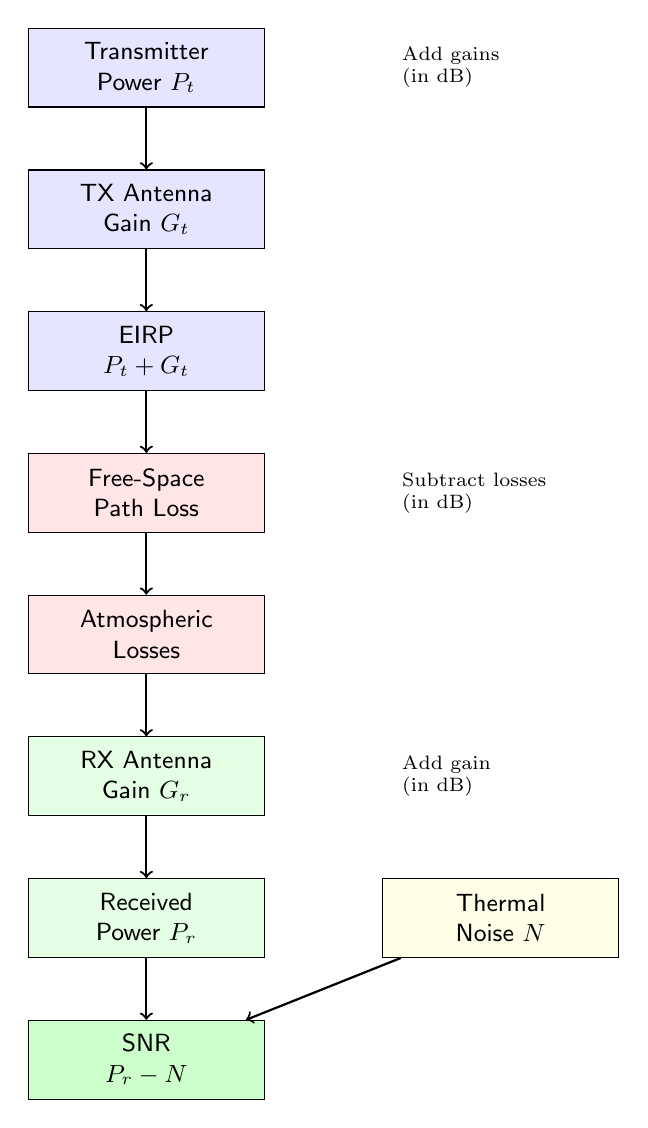
\begin{tikzpicture}[
  block/.style={rectangle, draw, minimum width=3cm, minimum height=1cm, font=\sffamily\small, align=center},
  arrow/.style={->, thick},
  node distance=1.8cm
]

% Transmitter side
\node[block, fill=blue!10] (tx) {Transmitter\\Power $P_t$};
\node[block, below of=tx, fill=blue!10] (txgain) {TX Antenna\\Gain $G_t$};
\node[block, below of=txgain, fill=blue!10] (eirp) {EIRP\\$P_t + G_t$};

% Propagation
\node[block, below of=eirp, fill=red!10] (fspl) {Free-Space\\Path Loss};
\node[block, below of=fspl, fill=red!10] (atmos) {Atmospheric\\Losses};

% Receiver side
\node[block, below of=atmos, fill=green!10] (rxgain) {RX Antenna\\Gain $G_r$};
\node[block, below of=rxgain, fill=green!10] (rxpower) {Received\\Power $P_r$};

% Noise and SNR
\node[block, right of=rxpower, node distance=4.5cm, fill=yellow!10] (noise) {Thermal\\Noise $N$};
\node[block, below of=rxpower, fill=green!20] (snr) {SNR\\$P_r - N$};

% Arrows
\draw[arrow] (tx) -- (txgain);
\draw[arrow] (txgain) -- (eirp);
\draw[arrow] (eirp) -- (fspl);
\draw[arrow] (fspl) -- (atmos);
\draw[arrow] (atmos) -- (rxgain);
\draw[arrow] (rxgain) -- (rxpower);
\draw[arrow] (rxpower) -- (snr);
\draw[arrow] (noise) -- (snr);

% Labels
\node[right of=tx, node distance=4.5cm, font=\scriptsize, text width=2.5cm] {Add gains\\(in dB)};
\node[right of=fspl, node distance=4.5cm, font=\scriptsize, text width=2.5cm] {Subtract losses\\(in dB)};
\node[right of=rxgain, node distance=4.5cm, font=\scriptsize, text width=2.5cm] {Add gain\\(in dB)};

\end{tikzpicture}
\end{center}

\subsection{Modulation Constellation Comparison}

\begin{center}
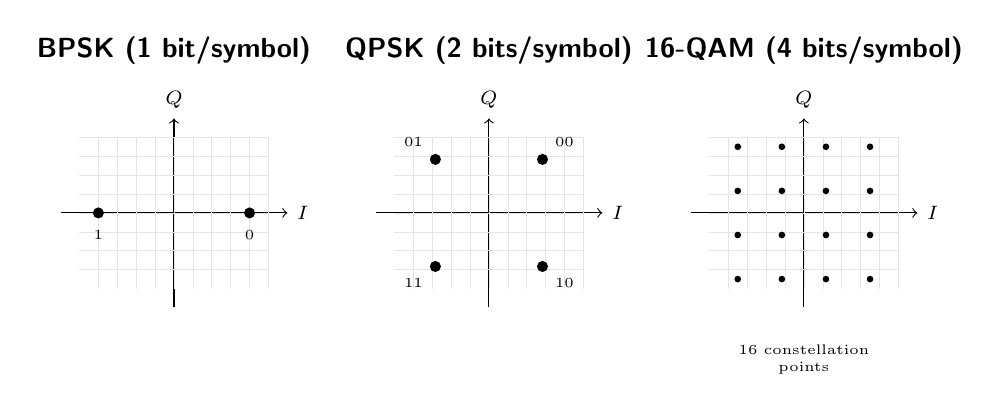
\begin{tikzpicture}[scale=0.8]

% BPSK
\begin{scope}[shift={(0,0)}]
\node[above,font=\sffamily\bfseries] at (0,2.2) {BPSK (1 bit/symbol)};
\draw[->] (-1.8,0) -- (1.8,0) node[right,font=\scriptsize] {$I$};
\draw[->] (0,-1.5) -- (0,1.5) node[above,font=\scriptsize] {$Q$};
\draw[very thin,gray!20] (-1.5,-1.2) grid[step=0.3] (1.5,1.2);
\fill[black] (-1.2,0) circle (2.5pt);
\fill[black] (1.2,0) circle (2.5pt);
\node[below=3pt,font=\tiny] at (-1.2,0) {1};
\node[below=3pt,font=\tiny] at (1.2,0) {0};
\end{scope}

% QPSK
\begin{scope}[shift={(5,0)}]
\node[above,font=\sffamily\bfseries] at (0,2.2) {QPSK (2 bits/symbol)};
\draw[->] (-1.8,0) -- (1.8,0) node[right,font=\scriptsize] {$I$};
\draw[->] (0,-1.5) -- (0,1.5) node[above,font=\scriptsize] {$Q$};
\draw[very thin,gray!20] (-1.5,-1.2) grid[step=0.3] (1.5,1.2);
\fill[black] (0.85,0.85) circle (2.5pt);
\fill[black] (-0.85,0.85) circle (2.5pt);
\fill[black] (-0.85,-0.85) circle (2.5pt);
\fill[black] (0.85,-0.85) circle (2.5pt);
\node[above right=1pt,font=\tiny] at (0.85,0.85) {00};
\node[above left=1pt,font=\tiny] at (-0.85,0.85) {01};
\node[below left=1pt,font=\tiny] at (-0.85,-0.85) {11};
\node[below right=1pt,font=\tiny] at (0.85,-0.85) {10};
\end{scope}

% 16-QAM
\begin{scope}[shift={(10,0)}]
\node[above,font=\sffamily\bfseries] at (0,2.2) {16-QAM (4 bits/symbol)};
\draw[->] (-1.8,0) -- (1.8,0) node[right,font=\scriptsize] {$I$};
\draw[->] (0,-1.5) -- (0,1.5) node[above,font=\scriptsize] {$Q$};
\draw[very thin,gray!20] (-1.5,-1.2) grid[step=0.3] (1.5,1.2);
% Grid of 16 points
\foreach \x in {-1.05,-0.35,0.35,1.05} {
  \foreach \y in {-1.05,-0.35,0.35,1.05} {
    \fill[black] (\x,\y) circle (1.5pt);
  }
}
\node[below=10pt,font=\tiny,align=center] at (0,-1.5) {16 constellation\\points};
\end{scope}

\end{tikzpicture}
\end{center}

\begin{keyconcept}
\textbf{Trade-off:} Higher-order modulation (more bits/symbol) requires higher SNR for the same BER. BPSK is most robust; 16-QAM is most efficient but needs clean channels.
\end{keyconcept}

\section{Worked Example: Complete Link Budget}
\label{sec:worked-example}

\textbf{Scenario:} Design a point-to-point microwave link for a cellular backhaul connection.

\subsection*{System Requirements}

\begin{tabular}{@{}ll@{}}
\toprule
\textbf{Parameter} & \textbf{Value} \\
\midrule
Distance & 10 km \\
Frequency & 18 GHz (Ku-band) \\
Data rate & 100 Mbps \\
Required BER & $10^{-6}$ \\
Modulation & 16-QAM \\
\bottomrule
\end{tabular}

\subsection*{Step 1: Free-Space Path Loss}

Using Equation~\ref{eq:fspl-km-mhz}:
\begin{equation}
\text{FSPL} = 20\log_{10}(10) + 20\log_{10}(18{,}000) + 32.45
\end{equation}
\begin{equation}
\text{FSPL} = 20 + 85.1 + 32.45 = 137.6\ \text{dB}
\end{equation}

\subsection*{Step 2: Link Budget}

Assuming:
\begin{itemize}
\item TX power: $P_t = 30$ dBm (1 W)
\item TX antenna gain: $G_t = 42$ dBi (1.2 m dish)
\item RX antenna gain: $G_r = 42$ dBi (1.2 m dish)
\item Atmospheric losses: $L_{\text{atm}} = 2$ dB
\item Miscellaneous losses: $L_{\text{misc}} = 3$ dB (cables, connectors)
\end{itemize}

Using Equation~\ref{eq:friis-db}:
\begin{equation}
P_r = P_t + G_t + G_r - \text{FSPL} - L_{\text{atm}} - L_{\text{misc}}
\end{equation}
\begin{equation}
P_r = 30 + 42 + 42 - 137.6 - 2 - 3 = -28.6\ \text{dBm}
\end{equation}

\subsection*{Step 3: Noise Power}

For bandwidth $B = 100$ MHz (approximately equal to data rate for 16-QAM), using Equation~\ref{eq:thermal-noise-db}:
\begin{equation}
N = -174 + 10\log_{10}(100 \times 10^6) = -174 + 80 = -94\ \text{dBm}
\end{equation}

Adding noise figure $NF = 4$ dB:
\begin{equation}
N_{\text{total}} = -94 + 4 = -90\ \text{dBm}
\end{equation}

\subsection*{Step 4: Signal-to-Noise Ratio}

Using Equation~\ref{eq:snr-db}:
\begin{equation}
\text{SNR} = P_r - N_{\text{total}} = -28.6 - (-90) = 61.4\ \text{dB}
\end{equation}

\subsection*{Step 5: Energy per Bit}

For 16-QAM, spectral efficiency $\eta \approx 4$ bps/Hz (4 bits/symbol).
\begin{equation}
\frac{E_b}{N_0} = \text{SNR} - 10\log_{10}(\eta)
\end{equation}
\begin{equation}
\frac{E_b}{N_0} = 61.4 - 10\log_{10}(4) = 61.4 - 6.0 = 55.4\ \text{dB}
\end{equation}

\subsection*{Step 6: BER Verification}

For 16-QAM, required $E_b/N_0 \approx 14$ dB for BER $= 10^{-6}$.

\textbf{Link margin:}
\begin{equation}
\text{Margin} = 55.4 - 14 = 41.4\ \text{dB}
\end{equation}

\begin{calloutbox}[colback=green!10,colframe=green!50!black]{Result}
\textbf{Link is viable with 41.4 dB margin.}

This substantial margin accounts for:
\begin{itemize}
\item Rain fade (up to 15 dB at 18 GHz in heavy rain)
\item Multipath fading (10--20 dB deep fades)
\item Equipment aging and temperature variations
\item Pointing errors and antenna misalignment
\end{itemize}

The link can reliably support 100 Mbps with 16-QAM modulation even in adverse weather conditions.
\end{calloutbox}

\section{Applications}
\label{sec:applications}

\subsection{Complete Link Budget Calculation}
\label{subsec:link-budget-example}

\begin{calloutbox}{Worked Example: 5G Base Station to Mobile}
\textbf{Given:}
\begin{itemize}
\item Frequency: 3.5 GHz
\item Distance: 500 m
\item TX power: 46 dBm (40 W)
\item TX antenna gain: 18 dBi (sector antenna)
\item RX antenna gain: 0 dBi (mobile phone)
\item Required SNR for 64-QAM: 20 dB
\item System bandwidth: 20 MHz
\end{itemize}

\textbf{Solution:}

\textbf{Step 1: Calculate FSPL}
\begin{align*}
\text{FSPL} &= 20\log_{10}(0.5) + 20\log_{10}(3500) + 32.45 \\
&= -6.02 + 70.88 + 32.45 = 97.31~\text{dB}
\end{align*}

\textbf{Step 2: Calculate received power}
\begin{align*}
P_r &= P_t + G_t + G_r - \text{FSPL} \\
&= 46 + 18 + 0 - 97.31 = -33.31~\text{dBm}
\end{align*}

\textbf{Step 3: Calculate noise floor}
\begin{align*}
N &= -174 + 10\log_{10}(20 \times 10^6) = -101~\text{dBm}
\end{align*}

\textbf{Step 4: Calculate SNR}
\begin{align*}
\text{SNR} &= P_r - N = -33.31 - (-101) = 67.69~\text{dB}
\end{align*}

\textbf{Result:} SNR = 67.69~dB $\gg$ 20~dB required. Link has 47.69~dB margin.
\end{calloutbox}

\subsection{Common System Parameters}
\label{subsec:common-systems}

\begin{table}[h]
\centering
\small
\begin{tabular}{@{}llll@{}}
\toprule
\textbf{System} & \textbf{Frequency} & \textbf{Modulation} & \textbf{Coding} \\
\midrule
WiFi 802.11g & 2.4 GHz & OFDM (BPSK--64QAM) & Convolutional \\
WiFi 802.11ax & 2.4/5 GHz & OFDM (BPSK--1024QAM) & LDPC \\
LTE & 700 MHz--2.6 GHz & OFDM (QPSK--256QAM) & Turbo \\
5G NR & 600 MHz--40 GHz & OFDM (QPSK--256QAM) & LDPC, Polar \\
GPS L1 & 1.575 GHz & BPSK & None (DSSS) \\
DVB-S2 & 10--12 GHz & 8PSK, 16/32APSK & LDPC + BCH \\
Bluetooth & 2.4 GHz & GFSK & None \\
LoRa & 433/868/915 MHz & CSS & Hamming \\
\bottomrule
\end{tabular}
\caption{Parameters for common wireless systems}
\label{tab:systems}
\end{table}

\section{Summary}

This formula reference card provides quick access to the essential equations for wireless communications analysis and design. Each formula has been presented with:

\begin{itemize}
\item \textbf{Clear definitions} of all variables with proper units
\item \textbf{Both linear and logarithmic} forms where applicable
\item \textbf{Worked examples} demonstrating practical calculations
\item \textbf{Cross-references} to detailed chapters for derivations
\item \textbf{Application context} for real-world systems
\end{itemize}

\begin{keyconcept}
Master these formulas and you have the foundation for analyzing any wireless communication system---from link budgets to error rates, from modulation schemes to channel effects.
\end{keyconcept}

For detailed derivations, proofs, and advanced topics, refer to the cross-referenced chapters throughout this book.
